\chapter{Execution, Capital Structure, and Durable Wealth}

This School of Hard Knocks interview, curated by LazyingArt LLC, is not a lecture in formal finance, but it still unfolds with a clear mathematical discipline. We are not given formulas first and examples second. We are given outcomes first, then the difficulty of reaching the people behind those outcomes, and only then the mechanisms. The chapter should therefore be read in the same order in which the lecture teaches: scale, access, case, doctrine. What emerges is a set of transformations rather than a single theory of money: small beginnings into enterprise value, founder-labor into transferability, operating cash into land and tenants, salary into family capital, and unrealized intention into a graveyard of unused possibilities.

\section{New York as a Wealth Field}

The lecture begins by putting wealth in front of us before it explains anything. A twenty-two-year-old millionaire appears. An NFL quarterback says that God made him a millionaire. A trucking operator says he began with two trucks and an empty warehouse and ended with real estate and a sale in the hundreds of millions. Another man is promised as having ``the best story in America.'' The function of this opening is not yet explanation. It is to establish the size of the field.

Only after this teaser does the host reset the scene. New York is named as the richest city in the world, the place where more billionaires, more millionaires, and more money move each day than anywhere else. The declared method is then simple and public: go straight to the source.

A useful chapter-wide ledger is therefore
\begin{align}
A_{\text{millionaire}}&=22\,\mathrm{yr},\\
V_{\text{Sweat}}&=\$400\times 10^6,\\
V_{\text{logistics}}&>\$500\times 10^6,\\
Y_{\text{Jameis,max}}&\approx \$25\times 10^6,\\
Y_{\text{metal,max}}&\in[\$60,\$70]\times 10^6.
\end{align}
These are not yet explanatory variables. They are markers of scale. The lecture's first move is to make us feel the pressure of the problem before it allows us to solve any part of it.

\begin{remark}
No validated mathematical screenshots survive for this lecture. The formulas and diagrams in this chapter are therefore transcript-backed reconstructions rather than frame-backed transcriptions.
\end{remark}

\section{Refusal, Persistence, and the Method of Access}

Once New York has been declared a wealth field, the lecture does something crucial: it makes access difficult. The host stops people in the street, gets refusals, gets people on phone calls, gets people who do not want to be delayed, and gets only one shallow partial answer from an angel investor. This matters because the lecture wants its knowledge to feel earned rather than prearranged.

The one numerical fragment that appears in this stretch is the familiar startup attrition estimate:
\begin{equation}
P(\text{fail by five years})\approx 0.8,\qquad
P(\text{survive by five years})\approx 0.2.
\end{equation}
The investor does not develop the claim. He says he would need to think about it. That hesitation is part of the point. We are not yet inside the explanatory layer of the lecture.

The host then turns to camera and gives the first recap: they have been trying all day; they are not going to stop; the richest city still has to be entered one interruption at a time. That recap tells us what the refusal montage means. It is not dead time. It is the proof that access is itself part of the argument.

\begin{figure}
\centering
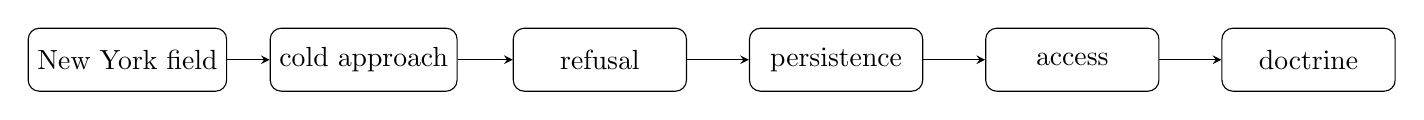
\begin{tikzpicture}[>=stealth]
\node[draw, rounded corners, minimum width=2.2cm, minimum height=0.8cm] (a) at (0,0) {New York field};
\node[draw, rounded corners, minimum width=2.2cm, minimum height=0.8cm] (b) at (3,0) {cold approach};
\node[draw, rounded corners, minimum width=2.2cm, minimum height=0.8cm] (c) at (6,0) {refusal};
\node[draw, rounded corners, minimum width=2.2cm, minimum height=0.8cm] (d) at (9,0) {persistence};
\node[draw, rounded corners, minimum width=2.2cm, minimum height=0.8cm] (e) at (12,0) {access};
\node[draw, rounded corners, minimum width=2.2cm, minimum height=0.8cm] (f) at (15,0) {doctrine};

\draw[->] (a) -- (b);
\draw[->] (b) -- (c);
\draw[->] (c) -- (d);
\draw[->] (d) -- (e);
\draw[->] (e) -- (f);
\end{tikzpicture}
\end{figure}

The first strong ``yes'' therefore matters structurally as well as biographically. It resolves the refusal sequence and opens the first full mechanism.

\section{Bootstrapping to a \$400 Million Exit}

The first sustained case comes from the founder of Sweat. The lecture first reconnects her to the opening teaser: she says she became a millionaire at twenty-two, and she gives the headline number quickly,
\begin{equation}
V_{\text{Sweat}}=\$400\times 10^6.
\end{equation}
Only after the headline number do we get the mechanism: she is from Australia, not from money, and the company was built without outside investors,
\begin{equation}
I_{\text{outside,Sweat}}=0.
\end{equation}

The lecture is careful about order here. It does not move directly from valuation to abstract business theory. It moves through boundary conditions. Australia is described as more relaxed; the United States as driven by hustle. The family did not provide the capital. The founding story appears to involve a backyard start, although the exact phrase in the transcript is unstable and should not be overquoted. Then comes the deeper point: in both life and business one is under no obligation to remain the same person one was yesterday. The lesson is not merely therapeutic. It is commercial. A business need not remain trapped inside the founder's first niche.

We can compress the chapter-wide commercial ladder as
\begin{equation}
K_{\text{start}} \to E_{\text{ops}} \to C_{\text{sale}} \to W_{\text{portfolio}},
\end{equation}
where \(K_{\text{start}}\) is an initially small or founder-built position, \(E_{\text{ops}}\) is operating execution, \(C_{\text{sale}}\) is a company that has become transferable enough to sell, and \(W_{\text{portfolio}}\) is what wealth becomes after the exit.

\subsection{Question \& Answer}

\paragraph{Question.} What makes a founder-built company actually sellable?

\paragraph{Answer.} The lecture's answer is not that a buyer merely wants growth. A buyer wants transferability.

\begin{definition}
We call \(R_{\text{sale}}\) the sale-readiness of a company: the degree to which the business can survive transfer without requiring the founder to remain its irreplaceable operating core.
\end{definition}

The founder says, in effect, that she made the company too dependent on herself. The host names the difficulty: key-man risk. The clean schematic relation is
\begin{equation}
R_{\text{sale}}\uparrow \qquad \text{as} \qquad D_{\text{founder}}\downarrow.
\end{equation}
This notation is our own, but it is faithful to the spoken logic. A founder-built company becomes more valuable as a transferable object when the founder ceases to be the only living mechanism inside it.

The lecture then makes a second move. It asks what money should do after the sale. The answer is not given as modern portfolio theory; it is given in concrete post-exit buckets, including a petrol station, property, and the market:
\begin{equation}
W_{\text{post-exit}}=W_{\text{gas}}+W_{\text{property}}+W_{\text{market}}.
\end{equation}
What matters is not the bookkeeping identity by itself, but the intuition behind it. The founder is excited not by abstraction, but by the sight of rent arriving from a gas station. The lecture likes this concreteness. It keeps money attached to visible cash flow.

The host then turns back to camera and tells us what he thinks has just happened: this was game for entrepreneurs. That recap should be kept. It tells us how the lecture wants the first case to land.

\section{From Trucks to Land to Tenants}

The second long case shifts the lecture out of founder culture and into operator arithmetic. The language changes at once. We leave apps and niches and enter the world of receivables, equipment, diesel, freight, land, and tenants. The operator begins with the roughest version of the small-start myth and then partially corrects it. He says he started from nothing; later he specifies that what he took over was a receivable of \$68.

That distinction matters. We should not simply replace the story by \(K_0=0\). The transcript gives us a more exact starting point:
\begin{align}
K_{\text{receivable},0}&=\$68,\\
N_{\text{trucks},0}&=2,\\
N_{\text{tenants}}&>1000.
\end{align}
The first quantity is a receivable, not necessarily liquid cash. But the large-scale transformation is unmistakable.

The lecture's central operator chain is
\begin{equation}
\text{trucking cash flow}\to \text{land}\to N_{\text{tenants}}\to \text{generational wealth}.
\end{equation}
This is the moment at which the chapter's title begins to earn itself. Rough work is converted into durable holdings. The trucking business is not treated as the terminal form of wealth. It is treated as the machine that generates land, and land is treated as the form in which wealth thickens and survives.

The operator is also unusually explicit about why he remained in an unglamorous line of work. He loved it. He loved the smell of diesel in the morning. Every morning felt like Christmas morning. That may sound rhetorical, but in the logic of the lecture it is a commercial fact. Daily enthusiasm sustains repetition, and repetition sustains compounding.

The lecture then widens the case by adding time, customers, and scale. The operator says that he dealt with major companies, that he brought freight to major retailers, and that land came into the story because the business needed it. The move is mechanical rather than mythic: operating scale demanded physical footprint, and physical footprint became real estate.

\subsection{Question \& Answer}

\paragraph{Question.} What actually creates wealth in real estate: leverage or resilience?

\paragraph{Answer.} The operator's answer is severe:
\begin{equation}
D_{\text{op}}=0.
\end{equation}
He calls himself a debt-free operator. The key word is not purity but rebound. If a mistake occurs, he says, one can recover. Those who are heavily leveraged may boast about how many buildings they own, but the lecture insists that apparent scale and real resilience are not the same object.

The host presses the point by asking how one can scale without borrowing, especially when even giant firms borrow. The operator's reply is that he never borrowed to run the business, with one stated exception: brand-new trucks. That exception then produces the cleanest worked mathematics in the lecture.

The three stated horizons are
\begin{equation}
T_{\text{expense}}=1\,\mathrm{yr},\qquad
T_{\text{pay}}=4\,\mathrm{yr},\qquad
T_{\text{use}}=10\,\mathrm{yr}.
\end{equation}

\begin{figure}
\centering
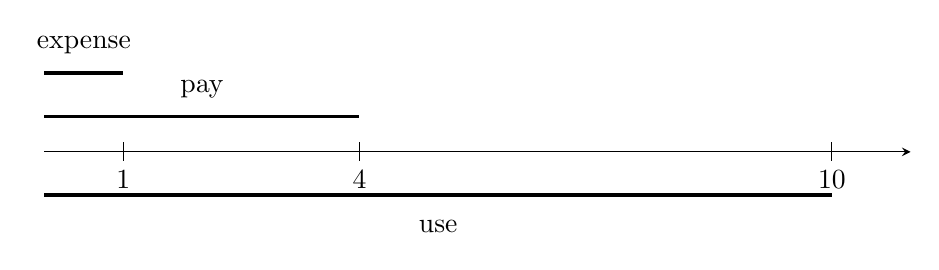
\begin{tikzpicture}[>=stealth]
\draw[->] (0,0) -- (11,0);
\draw (1,0.12) -- (1,-0.12) node[below]{1};
\draw (4,0.12) -- (4,-0.12) node[below]{4};
\draw (10,0.12) -- (10,-0.12) node[below]{10};

\draw[very thick] (0,1.0) -- (1,1.0);
\node at (0.5,1.35) {expense};

\draw[very thick] (0,0.45) -- (4,0.45);
\node at (2,0.8) {pay};

\draw[very thick] (0,-0.55) -- (10,-0.55);
\node at (5,-0.95) {use};
\end{tikzpicture}
\end{figure}

\paragraph{Worked example.}
The free-use interval after financing closes is
\begin{align}
T_{\text{free-use}}
&=T_{\text{use}}-T_{\text{pay}}\\
&=10-4\\
&=6\,\mathrm{yr}.
\end{align}
So on the speaker's own numbers, the truck remains in service for six years after the payment period ends. This is the lecture's clearest explicit derivation. The point is not depreciation theory. The point is that a durable productive asset can keep thickening cash flow after its financing burden has disappeared.

The lecture does not stop with debt and trucks. It turns again toward family. There are no free rolls in the bakery. The children must work. The business was sold because real estate was judged a better intergenerational vehicle. We should keep that sequence intact: operation, land, sale, transmission. The operator then adds another correlation, this time between bodily discipline and financial success. He answers ``one hundred percent'' when asked whether fitness and money are connected. The reasoning is simple: if one can govern the body daily, one has already learned something about repetition and self-command.

Then the lecture bends unexpectedly toward mortality. After the sale, the operator says, he had a massive heart attack. The quoted survival rates are stark:
\begin{equation}
p_{\text{hospital}}=0.11,\qquad
p_{\text{outside}}=0.05.
\end{equation}
These are not here to build a medical model. They are here because the lecture will not leave wealth alone. It pushes the argument through family, health, and finally a planning rule: be ten minutes early, think from Monday to Thursday, then think in five-year plans. The exact point is nested horizon discipline. One must live slightly ahead of the present in order to build beyond it.

\section{Execution Against the Graveyard}

After the logistics operator, the host stops and compresses the doctrine. Most people do not fail because they lack ideas. They fail because they never start. The graveyard metaphor is then introduced to give the doctrine a geometry. Unexecuted value is not merely absent. It is buried.

The lecture is almost diagrammatic already, so it is natural to write the contrast as a pair of state paths:
\begin{align}
\text{idea} &\to \text{excuse} \to \text{inaction},\\
\text{idea} &\to \text{first step} \to \text{execution} \to \text{learning}.
\end{align}

\begin{figure}
\centering
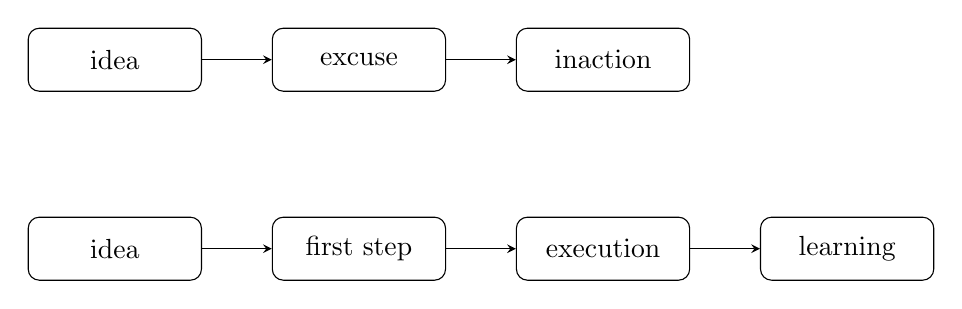
\begin{tikzpicture}[>=stealth]
\node[draw, rounded corners, minimum width=2.2cm, minimum height=0.8cm] (a1) at (0,1.2) {idea};
\node[draw, rounded corners, minimum width=2.2cm, minimum height=0.8cm] (a2) at (3.1,1.2) {excuse};
\node[draw, rounded corners, minimum width=2.2cm, minimum height=0.8cm] (a3) at (6.2,1.2) {inaction};

\node[draw, rounded corners, minimum width=2.2cm, minimum height=0.8cm] (b1) at (0,-1.2) {idea};
\node[draw, rounded corners, minimum width=2.2cm, minimum height=0.8cm] (b2) at (3.1,-1.2) {first step};
\node[draw, rounded corners, minimum width=2.2cm, minimum height=0.8cm] (b3) at (6.2,-1.2) {execution};
\node[draw, rounded corners, minimum width=2.2cm, minimum height=0.8cm] (b4) at (9.3,-1.2) {learning};

\draw[->] (a1) -- (a2);
\draw[->] (a2) -- (a3);

\draw[->] (b1) -- (b2);
\draw[->] (b2) -- (b3);
\draw[->] (b3) -- (b4);
\end{tikzpicture}
\end{figure}

The sponsor material that follows should be compressed but not deleted in spirit. Its structural role is to reduce the friction between idea and first step. The lecture is not making a deep claim about website software. It is preserving the doctrine that starting matters more than waiting for perfect readiness.

\section{High Income, Restraint, and Generational Choice}

A line from the opening teaser now returns in full: God made me a millionaire. In the full interview, however, the line is not left as a slogan. The host asks for the mechanism beneath the scale. We learn that Jameis Winston was twenty-one when he became a millionaire, that his biggest year was about twenty-five million dollars, and that the event marking that year was being drafted.

The lecture's important arithmetic here is not the salary alone but the partition rule:
\begin{align}
Y_{\text{Jameis,max}}&\approx \$25\times 10^6,\\
C_{\text{spend}}&\approx C_{\text{endorsements}},\\
C_{\text{game}}&\text{ is largely left untouched.}
\end{align}
This is the athlete's version of capital preservation. Current life runs off endorsement income; the primary game income is allowed to sit. The lecture is careful to place this rule before it turns toward family. Allocation precedes inheritance.

The second numerical contrast is temporal:
\begin{equation}
T_{\text{NFL}}=11\,\mathrm{yr},\qquad
T_{\text{NFL,avg}}\in[2,3]\,\mathrm{yr}.
\end{equation}
The host emphasizes how short the average professional career is. The player's eleven-year tenure is thus not just an anecdote; it is a durability outlier. When asked for the mechanism of that durability, he gives not a training protocol but a moral sequence: gratitude, hard work, and never giving up.

\subsection{Question \& Answer}

\paragraph{Question.} How does a rich family begin if one did not come from one?

\paragraph{Answer.} The lecture answers with a correction. The host says that a rich family will come from the player. The player sharpens the phrase: a wealthy family will come from him, through the choices and decisions that are made. The wording about generations in the transcript is conversational and somewhat unstable, but the intended structure is clear. Wealth begins here not as a single windfall but as repeated choice under restraint.

The lecture then asks what stabilizes those choices. The answer is faith. The player gives three rules of life: God, education, and the conviction that one can do what one sets one's mind to. The football translation is even simpler: never give up, never give up, never give up. We should not turn theology into fake algebra, but we should preserve the lecture's order. Faith comes first, then endurance, then the commercial result that money is less likely to outrun character.

The host's recap after the interview is also revealing. He says, in effect, that the lecture has moved beyond money. That is accurate. This section of the chapter is about what keeps a high-income life from becoming a high-income failure.

\section{Leverage, Collapse, Rebuilding, and Happiness After Money}

The final large case resolves the phrase from the teaser that promised ``the best story in America.'' The man says he got rich by shredding junk metal cars. Again the lecture uses rough work to puncture glamour. The numbers, however, are large:
\begin{align}
Y_{\text{metal,max}}&\in[\$60,\$70]\times 10^6,\\
V_{\text{firm}}&\approx \$10^9,\\
n_{\text{negotiation}}&=7.5/10.
\end{align}
The self-rating matters because it tells us that the lecture is not seeking mythic perfection. It values clear self-measurement.

The first doctrine here is that entrepreneurship is hard in ways that are not photogenic. Bloodshot eyes, little sleep, and a lack of glamour appear before the lecture allows any high-level abstraction. Then comes capital structure. This case differs sharply from the two earlier ones. The early business was financed with loans. The speaker says he was heavily leveraged. It was, in his own phrase, a mess. He later paid the loans off and says leverage can be part of growth, but just as clearly says that, at his current age, the leverage days are over. The lecture is not inconsistent here. It is distinguishing expansion tactics from durable equilibrium.

The next doctrine concerns paper. Watch the small print. Have someone review it. When you guarantee something, you are liable. This is the opposite of wealth mythology. It is contractual realism.

The chapter then enters its darkest interval. The exact legal vocabulary in the transcript is unstable, and we should not build technical banking notation out of it. What matters is that the speaker accepts guilt, is arrested, lives for years in the flux before prison, then spends a year in prison itself:
\begin{equation}
T_{\text{prison}}=1\,\mathrm{yr},\qquad
T_{\text{pre-prison flux}}\approx 4\,\mathrm{yr}.
\end{equation}
The lecture is precise about the emotional point. Prison is not only the sentence. It is also the period in which one knows what is coming and cannot yet resolve it.

\subsection{Question \& Answer}

\paragraph{Question.} What is the first actionable step after collapse?

\paragraph{Answer.} The lecture's answer is stripped down almost past elegance: stay focused and sacrifice. Do not wait to be rescued. Do not place yourself in situations where you already know the bad choice is waiting. When the host paraphrases the doctrine as ``nobody is coming to save you,'' the speaker agrees.

This answer is strengthened by an earlier sentence from the same section. When driving to prison, he asks his father for advice and receives not a long sermon but a blunt prohibition against self-pity. The lecture preserves this because it captures the transition from disaster to agency. Recovery is not presented as a financial formula. It is presented as a refusal to collapse inward.

The last turn of the lecture is about happiness. Do not believe your own hype. Do not believe your propaganda. Money is a mirage. The speaker says his greatest strength is that he can be happy with nothing. He does not deny that nice things are pleasant. He denies that they can carry the full weight of a life. This closes the chapter properly. Wealth appeared first as spectacle; it ends as something that must be subordinated to a person who can survive without spectacle.

\section{Summary}

The lecture proceeds by accumulation and correction. It shows us scale, then shows us how hard it is to access the people behind the scale, then lets those people convert anecdotes into mechanisms. Across the cases, the mechanisms rhyme without becoming identical.

\begin{itemize}
\item A founder-built company becomes sellable when founder dependence is reduced.
\item Unglamorous operating work can be converted into land, tenants, and intergenerational holdings.
\item Debt may speed growth, but resilience depends on how much room remains after error.
\item High income becomes family wealth only when it is partitioned, preserved, and governed by repeated choices.
\item Ideas become valuable only after execution crosses the threshold from excuse to action.
\end{itemize}

What gives the lecture its weight is that it never leaves money at the level of numbers. It repeatedly asks what structure can hold wealth, what habits can transmit it, and what sort of person remains after scale, danger, and recovery have all passed through the same life.